Preceding chapters have introduced methods for controllable synthesis of directed gaze shifts and demonstrated their use as building blocks of effective conversational behaviors for interactive virtual agents. The ability to synthesize humanlike behaviors in a controllable fashion is a necessary, but insufficient prerequisite for creating character animation.
To synthesize or author believable motion in a truly scalable way, one also requires the ability to apply that motion to characters with different designs and morphologies. The objective of character animation is to tell stories and those stories can involve characters of varying shapes, sizes, and species. In particular, stylized and anthropomorphic characters are found across many media, such as film and television animation, video games, and instructional content for children. As I already discussed in Section~\ref{sec:AnimatingStylizedCharacters}, automatically producing high-quality animation for such characters is a challenging and underexplored problem.

\begin{figure}
\centering
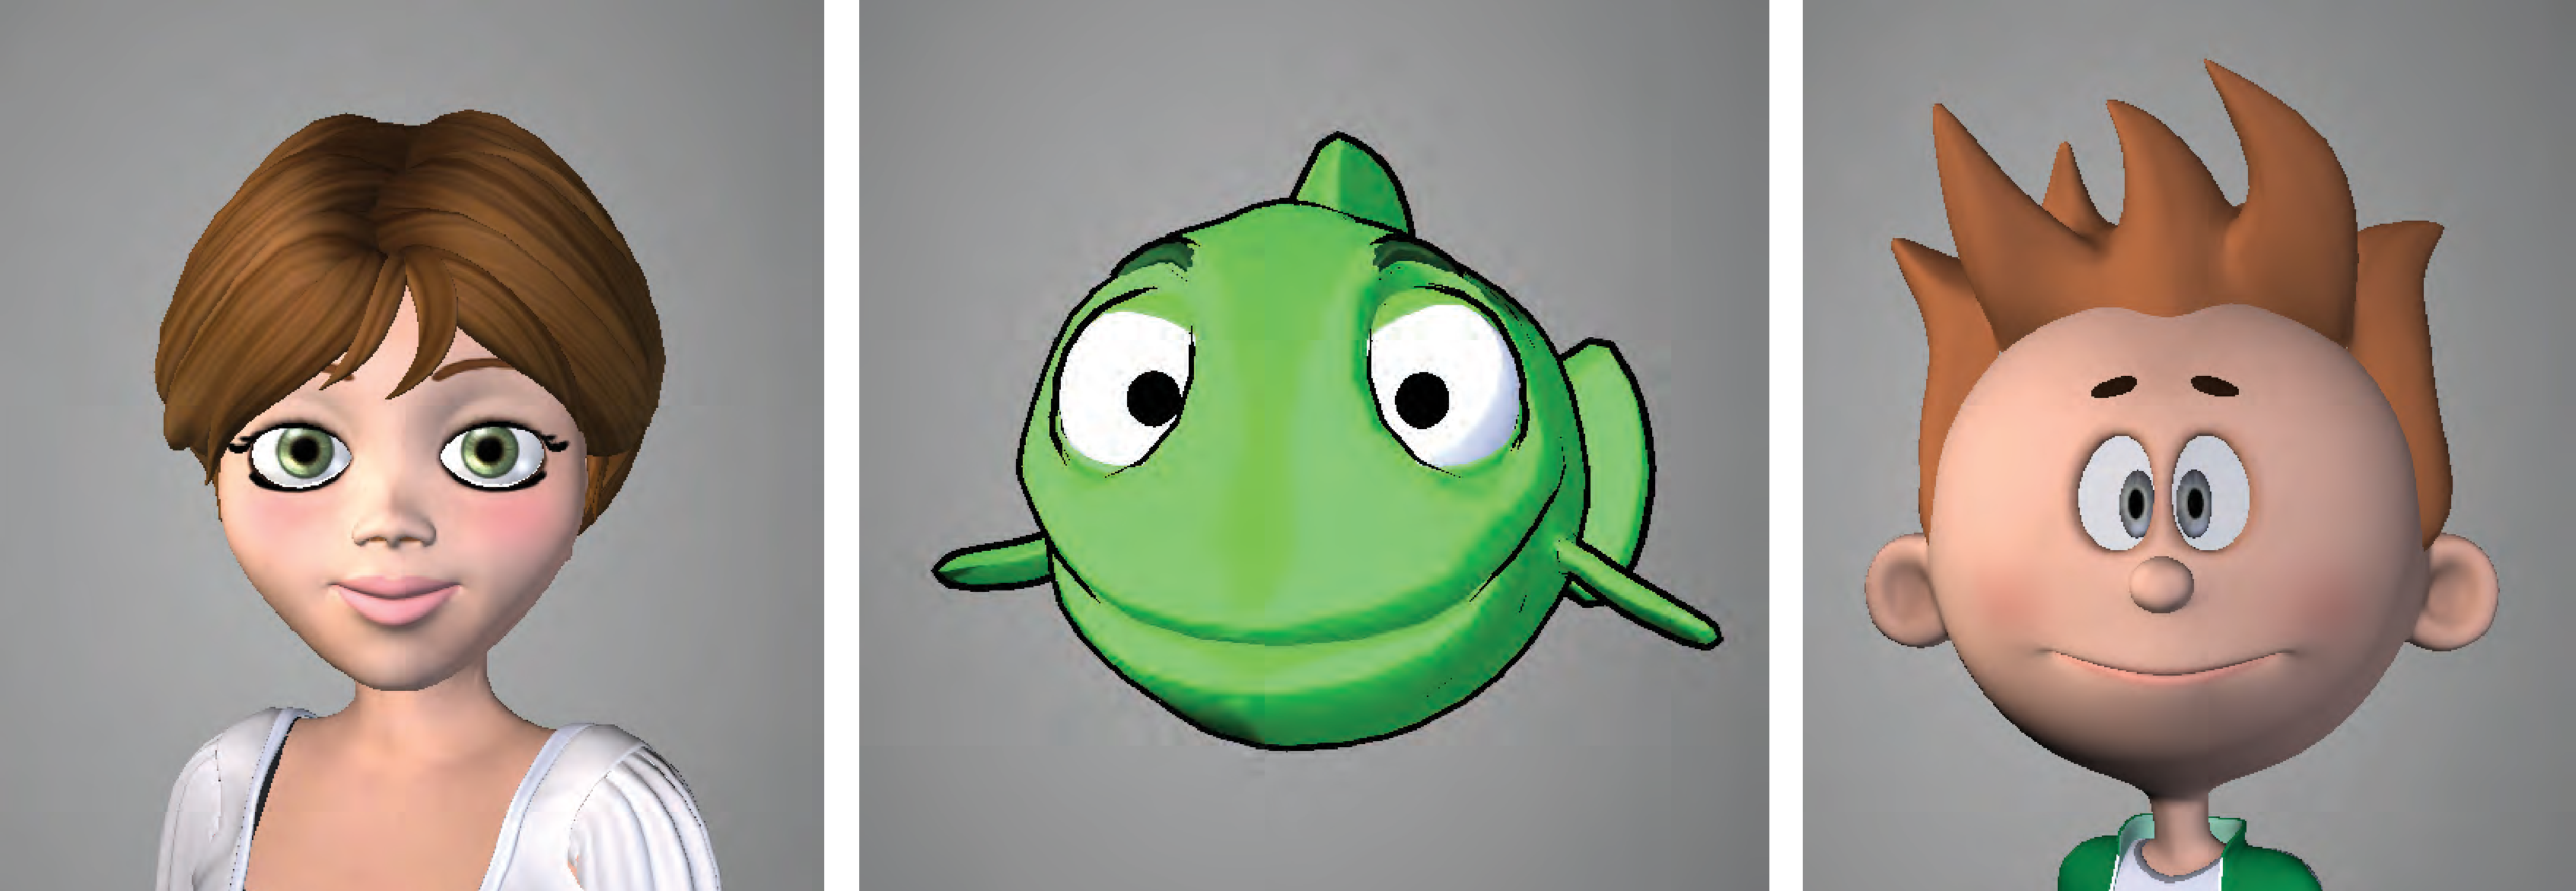
\includegraphics[width=0.85\textwidth]{stylizedgaze/Figures/StylizedCharacterExamples-small.pdf}
\caption{Examples of stylized characters. Characters 1 and 2 have large eyes and high inter-eye distance. Characters 2 and 3 have asymmetric eye motor range (OMR). Character 3 has narrow OMR and low inter-eye distance.}
\label{fig:StylizedCharacterExamples}
\end{figure}

The extent of this challenge is evident in the domain of gaze animation as well. Established methods for directed gaze animation have limited applicability to stylized characters; these methods are designed to simulate human gaze movements, so they implicitly incorporate human anatomic and neurophysiological constraints. Stylized characters tend to have exaggerated geometry with large and often asymmetrically shaped eyes such as those depicted in Figure~\ref{fig:StylizedCharacterExamples}. Applying models of realistic human gaze motion to such characters can result in aesthetically and communicatively poor animation. Enlarged and often asymmetric eye anatomy can magnify subtle phenomena of human gaze that are normally unnoticeable (e.g., cross-eyedness resulting from vergence) and lead to biologically implausible movements (e.g., one eye moving while the other is stationary.) Such gaze animation artifacts can appear unpleasant, distracting, and alter the communicative intent of the gaze behavior. In this chapter, I propose a set of online motion adaptation methods for reducing artifacts in gaze motion on stylized characters; I call these methods \emph{stylized gaze}. They are implemented as extensions of the gaze shift model described in Chapter~\ref{cha:GazeShiftModel}.

A secondary constraint of established gaze shift models is of a utilitarian variety: these models require the eyes to align exactly with the gaze target. The basis for this requirement seems obvious. For people, gaze has a perceptual utility---it enables us to see objects and other people. If human gaze always lines up with its target in the environment, why not require the same of virtual characters' gaze?
However, when we look beyond everyday usage of gaze, we realize there are many situations when people do not look in order to see.
In visual storytelling media, such as theater, film, and cartoon animation, the primary purpose of gaze is to communicate ideas to the audience. The actor's line of sight does not always align with the target they are ``looking'' at. Actors often look only in the general direction of the target, while maintaining the orientation of their body toward the camera or audience. The audience can more clearly see what the actor is attending to, even if their line of sight is not actually aligned with the target.
I dub this partially aligned, viewer-oriented gaze behavior \emph{performative gaze}. The technique has a basis in human perception---people are notoriously imprecise at estimating the gaze direction of others, unless they themselves are being looked at~\citep{argyle1976gaze}. In this chapter, I propose a method for automatic adaptation of gaze shift motion relative to the viewpoint (i.e., camera position), allowing an animator to achieve performative gaze through the manipulation of a single parameter.

The remainder of the chapter is organized as follows: I give an overview of animation artifacts that occur when applying humanlike gaze shift movements to stylized characters (Section~\ref{sec:StylizedGazeArtifacts}), I present the stylized gaze methods for the adaptation of gaze shift movements to stylized characters (Section~\ref{sec:StylizedGazeAdaptation}), and I present the performative gaze method for adaptation of gaze shift movements relative to the viewpoint (Section~\ref{sec:PerformativeGaze}). Finally, I demonstrate how the proposed methods lead to reduction of undesirable artifacts in gaze motion without compromising the communicative effectiveness of gaze shifts (Sections~\ref{sec:StylizedGazeEvaluation1} and~\ref{sec:StylizedGazeEvaluation2}). 